\chapter{Elder Heliosystem Memory Architecture}

\section{Introduction to Elder Memory Organization}

The Elder Heliosystem implements a novel memory architecture that fundamentally differs from traditional neural network implementations. Rather than storing information in a sequential token-based format or through fixed-weight matrices, the Elder system organizes knowledge through phase-encoded orbital representations. This chapter details the precise memory map of the Elder Heliosystem as it exists in both system memory and computational accelerator memory.

\section{Memory Hierarchy Overview}

The Elder Heliosystem employs a hierarchical memory organization that mirrors its orbital computational structure:

\begin{figure}[h]
\centering
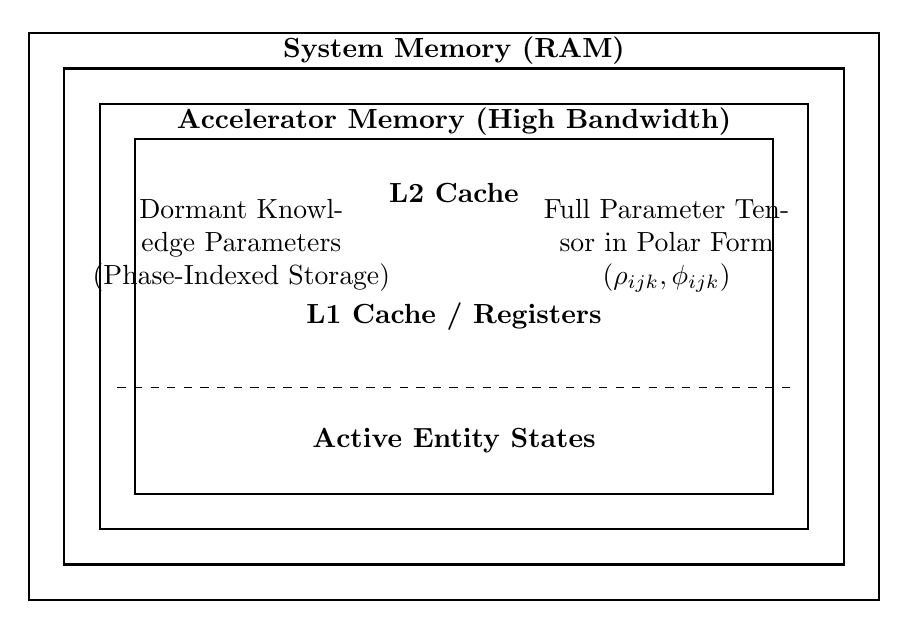
\begin{tikzpicture}[scale=0.9]
% Memory hierarchy overview
\draw[thick] (0,0) rectangle (12,8);
\draw[thick] (0.5,0.5) rectangle (11.5,7.5);
\draw[thick] (1,1) rectangle (11,7);
\draw[thick] (1.5,1.5) rectangle (10.5,6.5);

% Labels
\node at (6,7.75) {\textbf{System Memory (RAM)}};
\node at (6,6.75) {\textbf{Accelerator Memory (High Bandwidth)}};
\node at (6,5.75) {\textbf{L2 Cache}};
\node at (6,4) {\textbf{L1 Cache / Registers}};

% Memory contents
\draw[dashed] (1.25,3) -- (10.75,3);
\node at (6,2.25) {\textbf{Active Entity States}};

% Active vs dormant regions
\node[text width=5cm, align=center] at (3,5) {Dormant Knowledge Parameters \\ (Phase-Indexed Storage)};
\node[text width=5cm, align=center] at (9,5) {Full Parameter Tensor in Polar Form \\ $(\rho_{ijk}, \phi_{ijk})$};

\end{tikzpicture}
\caption{Elder Heliosystem Memory Hierarchy}
\end{figure}

\section{System Memory (RAM) Organization}

The Elder Heliosystem's system memory is organized into distinct regions, each serving a specific function:

\begin{table}[h]
\centering
\small
\begin{tabular}{|p{3.5cm}|p{3cm}|p{3cm}|p{4cm}|}
\hline
\textbf{Memory Region} & \textbf{Size} & \textbf{Access Pattern} & \textbf{Contents} \\
\hline
Entity State Buffer & 256 KB & High-frequency random access & Complete states of Elder, Mentors, and Erudites \\
\hline
Phase-Indexed Parameter Table & 16-64 MB & Sparse, phase-driven access & Mapping from phase values to parameter indices \\
\hline
Parameter Storage (Dormant) & 1-8 GB & Batch retrieval on phase activation & Majority of knowledge parameters in compressed format \\
\hline
Input/Output Buffers & 128-512 MB & Sequential & Streaming data being processed \\
\hline
Phase Transition Records & 64 MB & Append-only & Historical record of phase transitions for analysis \\
\hline
Executables \& Runtime & 128 MB & Code access & System code, runtime libraries \\
\hline
\end{tabular}
\caption{System Memory (RAM) Organization}
\end{table}

\subsection{Entity State Buffer}

The Entity State Buffer contains the dynamic state of all entities in the system:

\begin{equation}
\text{Size}_{\text{EntityBuffer}} = N_{\text{Elder}} \times S_{\text{Elder}} + N_{\text{Mentor}} \times S_{\text{Mentor}} + N_{\text{Erudite}} \times S_{\text{Erudite}}
\end{equation}

Where:
\begin{itemize}
    \item $N_{\text{Elder}} = 1$, $S_{\text{Elder}} = 53$ bytes (optimized representation)
    \item $N_{\text{Mentor}} = 32$, $S_{\text{Mentor}} = 53$ bytes (optimized representation)
    \item $N_{\text{Erudite}} = 4,096$, $S_{\text{Erudite}} = 29$ bytes (optimized representation)
\end{itemize}

Yielding approximately 121 KB for entity states, with additional memory reserved for growth and alignment.

\subsection{Phase-Indexed Parameter Table}

This critical data structure enables the system's $\mathcal{O}(1)$ memory efficiency. It maps phase values to parameter indices, allowing sparse activation:

\begin{tcolorbox}[colback=LightGray, colframe=DarkGray, title=Phase-Indexed Parameter Table Structure, fonttitle=\bfseries]
\begin{verbatim}
struct PhaseIndexEntry {
    PhaseValue phase;          // 2 bytes (quantized phase)  
    uint32_t parameterIndex;   // 4 bytes (index into parameter storage)
    uint16_t domainID;         // 2 bytes (associated domain)
    uint8_t activationStrength; // 1 byte (activation coefficient)
};  // 9 bytes per entry
\end{verbatim}
\end{tcolorbox}

With approximately 7 million phase index entries, this table requires around 63 MB of memory. It is organized as a hash table with phase values as keys for $\mathcal{O}(1)$ lookup time.

\section{Accelerator Memory Organization}

High-bandwidth accelerator memory stores actively used parameters and computational structures:

\begin{table}[h]
\centering
\small
\begin{tabular}{|p{3.5cm}|p{2.5cm}|p{3.2cm}|p{4.3cm}|}
\hline
\textbf{Accelerator Region} & \textbf{Size} & \textbf{Access Pattern} & \textbf{Contents} \\
\hline
Active Parameter Tensor & 64-256 MB & Phase-localized & Currently active parameters based on Elder phase \\
\hline
Entity State Mirror & 256 KB & Continuous update & Synchronized copy of system Entity State Buffer \\
\hline
Orbital Dynamics Engine & 32 MB & Compute-intensive & Computational structures for orbital updates \\
\hline
Phase Transformation Unit & 16 MB & Compute-intensive & Operators for phase-based activations \\
\hline
Sparse Activation Masks & 8 MB & Bit-parallel & Binary masks for parameter activation \\
\hline
Output Accumulation Buffer & 32-128 MB & Reduction operations & Intermediate results of computation \\
\hline
\end{tabular}
\caption{Accelerator Memory Organization}
\end{table}

\subsection{Active Parameter Tensor}

The active parameter tensor contains only the subset of parameters relevant to the current phase region:

\begin{equation}
\text{ActiveParams} = \{ \theta_i \mid |\phi_i - \phi_{\text{Elder}}| < \Delta\phi_{\text{threshold}} \}
\end{equation}

With a typical sparsity factor of $10^{-4}$, only about 120,000 parameters are active at any given time, requiring approximately 120 MB of memory (assuming complex-valued parameters stored in polar form).

\begin{tcolorbox}[colback=LightGray, colframe=DarkGray, title=Active Parameter Representation, fonttitle=\bfseries]
\begin{verbatim}
struct ActiveParameter {
    float magnitude;      // 4 bytes (ρ value)
    uint16_t phase;       // 2 bytes (quantized φ value)
    uint16_t domainMask;  // 2 bytes (domain applicability)
    uint32_t metadata;    // 4 bytes (additional parameter-specific data)
};  // 12 bytes per active parameter
\end{verbatim}
\end{tcolorbox}

\section{Memory Management Dynamics}

The Elder Heliosystem employs specialized memory management strategies to maintain its $\mathcal{O}(1)$ memory scaling:

\subsection{Phase-Based Parameter Swapping}

As the Elder phase evolves, parameters move between dormant storage and the active parameter tensor:

\begin{algorithm}
\caption{Phase-Based Parameter Management}
\begin{algorithmic}[1]
\State \textbf{Initialize} ActiveParameterSet $\gets \emptyset$
\State \textbf{Initialize} $\phi_{\text{Elder}} \gets 0.0$

\While{processing input}
    \State Update $\phi_{\text{Elder}}$ based on input and orbital dynamics
    \State Identify parameters entering activation range: $P_{\text{in}} = \{\theta_i \mid |\phi_i - \phi_{\text{Elder}}| < \Delta\phi_{\text{threshold}} \land \theta_i \notin \text{ActiveParameterSet}\}$
    \State Identify parameters leaving activation range: $P_{\text{out}} = \{\theta_i \mid |\phi_i - \phi_{\text{Elder}}| \geq \Delta\phi_{\text{threshold}} \land \theta_i \in \text{ActiveParameterSet}\}$
    
    \State Load $P_{\text{in}}$ from dormant storage to active parameter tensor
    \State Remove $P_{\text{out}}$ from active parameter tensor
    
    \State Update $\text{ActiveParameterSet} \gets (\text{ActiveParameterSet} \setminus P_{\text{out}}) \cup P_{\text{in}}$
    \State Perform computation using $\text{ActiveParameterSet}$
\EndWhile
\end{algorithmic}
\end{algorithm}

This dynamic swapping strategy ensures that memory usage remains constant regardless of the total sequence length being processed.

\subsection{Phase Locality Optimization}

The Elder Heliosystem organizes parameters to maximize phase locality, placing related parameters at similar phase values. This optimization enhances computational efficiency:

\begin{equation}
\text{PhaseLocality}(\phi_i, \phi_j) = \begin{cases}
1 - \frac{|\phi_i - \phi_j|}{\pi}, & \text{if } |\phi_i - \phi_j| \leq \pi \\
1 - \frac{2\pi - |\phi_i - \phi_j|}{\pi}, & \text{if } |\phi_i - \phi_j| > \pi
\end{cases}
\end{equation}

Parameters with high semantic or functional relatedness are assigned phases with high phase locality, ensuring they are activated together.

\section{Memory Footprint Analysis}

\subsection{Typical Configuration Memory Requirements}

For a standard Elder Heliosystem configuration with 1 Elder, 32 Mentors, and 4,096 Erudites:

\begin{table}[h]
\centering
\begin{tabular}{|l|r|r|}
\hline
\textbf{Memory Component} & \textbf{System Memory (RAM)} & \textbf{Accelerator Memory} \\
\hline
Entity States & 256 KB & 256 KB \\
Phase-Index Structure & 64 MB & --- \\
Knowledge Parameters & 4,096 MB & 128 MB (active subset) \\
Computational Buffers & 512 MB & 128 MB \\
Runtime \& Executables & 128 MB & 32 MB \\
\hline
\textbf{Total} & \textbf{4,800 MB} & \textbf{288 MB} \\
\hline
\end{tabular}
\caption{Memory Footprint Summary}
\end{table}

\subsection{Critical Advantage: Constant Scaling with Sequence Length}

Unlike transformer models where memory requirements grow with sequence length, the Elder Heliosystem maintains constant memory usage regardless of input duration:

\begin{figure}[h]
\centering
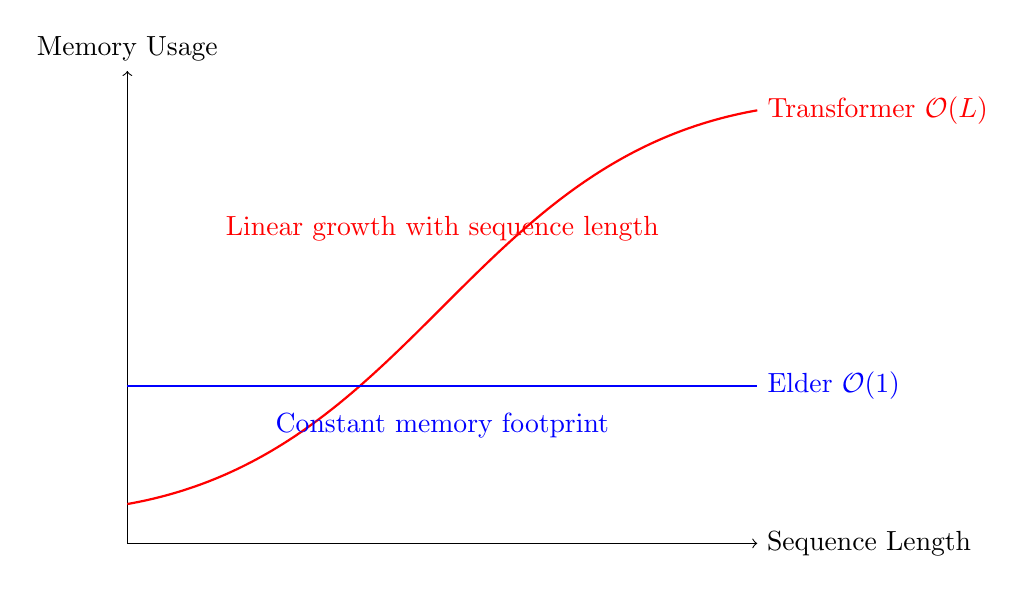
\begin{tikzpicture}
% Axes
\draw[->] (0,0) -- (8,0) node[right] {Sequence Length};
\draw[->] (0,0) -- (0,6) node[above] {Memory Usage};

% Transformer scaling
\draw[thick, color=red] (0,0.5) to[out=10, in=190] (8,5.5) node[right] {Transformer $\mathcal{O}(L)$};

% Elder scaling
\draw[thick, color=blue] (0,2) -- (8,2) node[right] {Elder $\mathcal{O}(1)$};

% Annotations
\node[color=blue] at (4,1.5) {Constant memory footprint};
\node[color=red] at (4,4) {Linear growth with sequence length};

\end{tikzpicture}
\caption{Memory Scaling Comparison: Elder vs. Transformer}
\end{figure}

\section{Memory Access Patterns}

The Elder Heliosystem exhibits distinctive memory access patterns optimized for its phase-based computational model:

\subsection{Phase-Driven Access}

Memory access is primarily dictated by the Elder phase value, which determines which parameters are active:

\begin{equation}
\text{Access}_t(\theta_i) = \begin{cases}
\text{true}, & \text{if } |\phi_i - \phi_{\text{Elder}}(t)| < \Delta\phi_{\text{threshold}} \\
\text{false}, & \text{otherwise}
\end{cases}
\end{equation}

This results in a circular traversal pattern through parameter space as the Elder phase evolves, rather than the sequential access patterns seen in traditional models.

\subsection{Orbital Dynamics Memory Flow}

The orbital dynamics of the system create a natural memory hierarchy, where information flows between entities based on their orbital relationships:

\begin{itemize}
    \item \textbf{Elder → Mentor Flow:} Phase-based coupling between Elder and Mentors
    \item \textbf{Mentor → Erudite Flow:} Domain-specific information transfer to specialized processing units
    \item \textbf{Cross-Orbital Transfer:} Information exchange between Mentors via phase coupling
\end{itemize}

This memory flow architecture enables the system to maintain coherence across domains while preserving the efficiency of localized computations.

\section{Implementation Considerations}

When implementing the Elder Heliosystem on physical hardware, several optimizations are critical:

\begin{itemize}
    \item \textbf{Phase Indexing:} Efficient phase-indexed lookup tables with uniform bucket distribution
    \item \textbf{Parameter Prefetching:} Anticipatory loading of parameters that will soon enter the active phase window
    \item \textbf{Entity Alignment:} Memory-aligned entity state storage for efficient vector operations
    \item \textbf{Phase Quantization:} Adaptive precision for phase values based on parameter sensitivity
    \item \textbf{Sparse Matrix Operations:} Optimized computation on sparse, phase-local parameter subsets
\end{itemize}

\section{Conclusion}

The memory architecture of the Elder Heliosystem represents a fundamental departure from traditional machine learning memory models. By organizing knowledge in phase space rather than sequence space, it achieves $\mathcal{O}(1)$ memory scaling with respect to sequence length. This architecture enables processing of unbounded context while maintaining a constant, manageable memory footprint, making it uniquely suited for continuous, long-term learning across multiple domains.